\documentclass[tikz,border=5pt]{standalone}
\usepackage[T1]{fontenc}
\usepackage[scaled=0.92]{helvet}
\usepackage{amsmath,amssymb}
\usepackage{tikz}
\usetikzlibrary{arrows.meta,positioning,shapes.geometric,shapes.misc,calc,fit,backgrounds}

\begin{document}
\sffamily
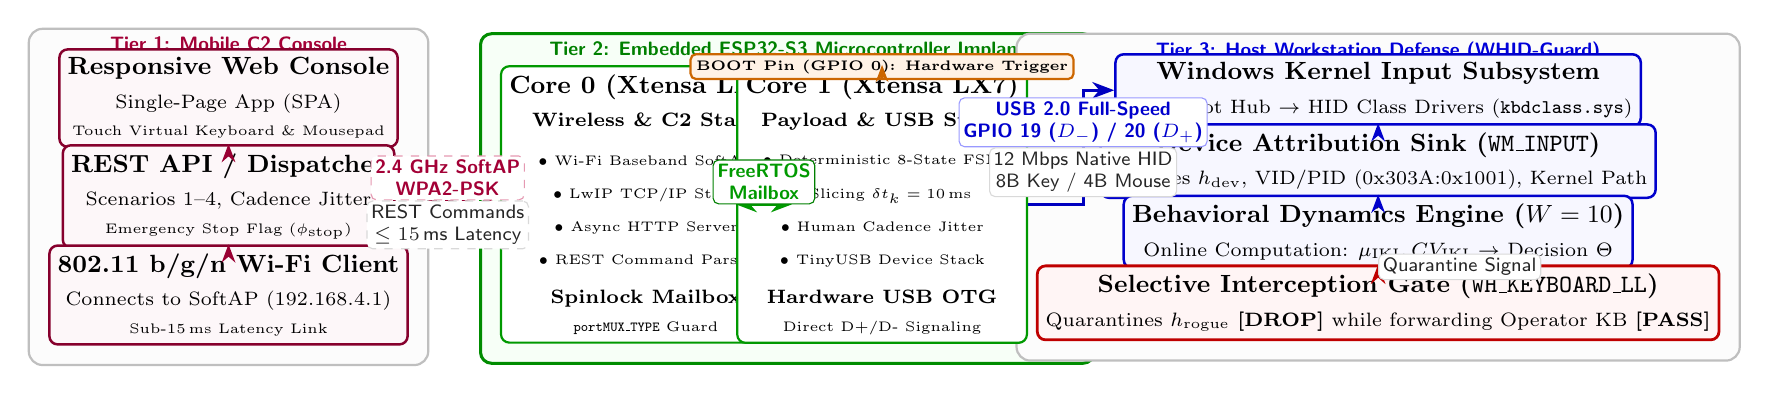
\begin{tikzpicture}[
    >=Stealth,
    font=\small,
    % Outer Container Styles
    tier_box/.style={
        rectangle,
        rounded corners=5pt,
        draw=gray!50,
        line width=0.8pt,
        fill=gray!2,
        inner sep=6pt
    },
    % Module Card Styles
    c2_card/.style={
        rectangle,
        rounded corners=3pt,
        draw=purple!70!black,
        line width=0.9pt,
        fill=purple!3!white,
        minimum width=3.3cm,
        minimum height=0.88cm,
        inner sep=3pt,
        align=center
    },
    soc_chip/.style={
        rectangle,
        rounded corners=4pt,
        draw=green!55!black,
        line width=1.1pt,
        fill=green!3!white,
        inner sep=6pt
    },
    core_box/.style={
        rectangle,
        rounded corners=3pt,
        draw=green!60!black,
        line width=0.8pt,
        fill=white,
        minimum width=2.4cm,
        minimum height=2.6cm,
        inner sep=3pt,
        align=center
    },
    host_card/.style={
        rectangle,
        rounded corners=3pt,
        draw=blue!80!black,
        line width=0.9pt,
        fill=blue!3!white,
        minimum width=4.9cm,
        minimum height=0.82cm,
        inner sep=3pt,
        align=center
    },
    gate_card/.style={
        rectangle,
        rounded corners=3pt,
        draw=red!75!black,
        line width=1.0pt,
        fill=red!4!white,
        minimum width=4.9cm,
        minimum height=0.82cm,
        inner sep=3pt,
        align=center
    },
    % Badges
    lbl/.style={
        font=\sffamily\scriptsize,
        fill=white,
        draw=gray!30,
        line width=0.4pt,
        rounded corners=2pt,
        inner sep=1.5pt,
        align=center,
        text=black!85
    },
    lbl_purple/.style={
        font=\sffamily\scriptsize\bfseries,
        fill=white,
        draw=purple!40,
        line width=0.4pt,
        rounded corners=2pt,
        inner sep=1.5pt,
        align=center,
        text=purple!85!black
    },
    lbl_green/.style={
        font=\sffamily\scriptsize\bfseries,
        fill=white,
        draw=green!50!black,
        line width=0.4pt,
        rounded corners=2pt,
        inner sep=1.5pt,
        align=center,
        text=green!60!black
    },
    lbl_blue/.style={
        font=\sffamily\scriptsize\bfseries,
        fill=white,
        draw=blue!40,
        line width=0.4pt,
        rounded corners=2pt,
        inner sep=1.5pt,
        align=center,
        text=blue!80!black
    }
]

% ==============================================================================
% TIER 1: Out-of-Band Wireless Mobile Controller (C2) (x = 0 to 3.5)
% ==============================================================================
\node[c2_card] (c2_web)  at (1.7, 1.25) {\textbf{Responsive Web Console}\\[1pt]\scriptsize Single-Page App (SPA)\\[-1pt]\tiny Touch Virtual Keyboard \& Mousepad};
\node[c2_card] (c2_api)  at (1.7, 0.0)  {\textbf{REST API / Dispatcher}\\[1pt]\scriptsize Scenarios 1--4, Cadence Jitter\\[-1pt]\tiny Emergency Stop Flag ($\phi_{\text{stop}}$)};
\node[c2_card] (c2_wifi) at (1.7, -1.25) {\textbf{802.11 b/g/n Wi-Fi Client}\\[1pt]\scriptsize Connects to SoftAP ($192.168.4.1$)\\[-1pt]\tiny Sub-15\,ms Latency Link};

\draw[->, line width=0.8pt, draw=purple!80!black] (c2_web.south) -- (c2_api.north);
\draw[->, line width=0.8pt, draw=purple!80!black] (c2_api.south) -- (c2_wifi.north);

\begin{scope}[on background layer]
    \node[tier_box, fit=(c2_web) (c2_api) (c2_wifi), inner sep=7pt] (tier1_bg) {};
    \node[anchor=north, font=\sffamily\bfseries\scriptsize, text=purple!85!black] at (tier1_bg.north) {Tier 1: Mobile C2 Console};
\end{scope}

% ==============================================================================
% TIER 2: Embedded ESP32-S3 Hardware Implant (x = 5.8 to 11.4)
% ==============================================================================
% Core 0 Box
\node[core_box] (core0) at (7.0, -0.1) {
    \textbf{Core 0 (Xtensa LX7)}\\[1pt]\scriptsize \textbf{Wireless \& C2 Stack}\\[3pt]
    \tiny $\bullet$ Wi-Fi Baseband SoftAP\\[1pt]
    \tiny $\bullet$ LwIP TCP/IP Stack\\[1pt]
    \tiny $\bullet$ Async HTTP Server\\[1pt]
    \tiny $\bullet$ REST Command Parser\\[3pt]
    \scriptsize \textbf{Spinlock Mailbox}\\[-1pt]
    \tiny \texttt{portMUX\_TYPE} Guard
};

% Core 1 Box
\node[core_box] (core1) at (10.0, -0.1) {
    \textbf{Core 1 (Xtensa LX7)}\\[1pt]\scriptsize \textbf{Payload \& USB Stack}\\[3pt]
    \tiny $\bullet$ Deterministic 8-State FSM\\[1pt]
    \tiny $\bullet$ Slicing $\delta t_k=10$\,ms\\[1pt]
    \tiny $\bullet$ Human Cadence Jitter\\[1pt]
    \tiny $\bullet$ TinyUSB Device Stack\\[3pt]
    \scriptsize \textbf{Hardware USB OTG}\\[-1pt]
    \tiny Direct D+/D- Signaling
};

% Spinlock communication between cores
\draw[<->, line width=1.0pt, draw=green!60!black] (core0.east) -- node[above, lbl_green] {FreeRTOS\\Mailbox} (core1.west);

% Physical Push-Button on SoC
\node[rectangle, rounded corners=2pt, draw=orange!80!black, fill=orange!10!white, line width=0.8pt, inner sep=2pt] (boot_btn) at (10.0, 1.65) {\tiny\textbf{BOOT Pin (GPIO 0): Hardware Trigger}};
\draw[->, line width=0.7pt, draw=orange!80!black] (boot_btn.south) -- (core1.north);

% Pinout on SoC East edge
\coordinate (pin_usb) at (11.2, -0.1);

\begin{scope}[on background layer]
    \node[soc_chip, fit=(core0) (core1) (boot_btn), inner sep=7pt] (soc_bg) {};
    \node[anchor=north, font=\sffamily\bfseries\scriptsize, text=green!50!black] at (soc_bg.north) {Tier 2: Embedded ESP32-S3 Microcontroller Implant};
\end{scope}

% ==============================================================================
% RF Wireless Link (Tier 1 -> Tier 2)
% ==============================================================================
\draw[->, line width=1.1pt, draw=purple!80!black, dashed] (c2_api.east) -- (core0.west)
    node[pos=0.5, above, lbl_purple] {2.4 GHz SoftAP\\WPA2-PSK}
    node[pos=0.5, below, lbl] {REST Commands\\$\le 15$\,ms Latency};

% ==============================================================================
% TIER 3: Host Workstation & WHID-Guard Defense (x = 13.8 to 18.8)
% ==============================================================================
\node[host_card] (host_kernel) at (16.3, 1.35) {\textbf{Windows Kernel Input Subsystem}\\[1pt]\scriptsize USB Root Hub $\rightarrow$ HID Class Drivers (\texttt{kbdclass.sys})};

\node[host_card] (host_raw) at (16.3, 0.45) {\textbf{Device Attribution Sink (\texttt{WM\_INPUT})}\\[1pt]\scriptsize Resolves $h_{\text{dev}}$, VID/PID (0x303A:0x1001), Kernel Path};

\node[host_card] (host_engine) at (16.3, -0.45) {\textbf{Behavioral Dynamics Engine ($W=10$)}\\[1pt]\scriptsize Online Computation: $\mu_{\text{IKI}}, CV_{\text{IKI}}$ $\rightarrow$ Decision $\Theta$};

\node[gate_card] (host_gate) at (16.3, -1.35) {\textbf{Selective Interception Gate (\texttt{WH\_KEYBOARD\_LL})}\\[1pt]\scriptsize Quarantines $h_{\text{rogue}}$ \textbf{[DROP]} while forwarding Operator KB \textbf{[PASS]}};

% Host Internal Dataflows
\draw[->, line width=0.8pt, draw=blue!80!black] (host_kernel.south) -- (host_raw.north);
\draw[->, line width=0.8pt, draw=blue!80!black] (host_raw.south) -- (host_engine.north);
\draw[->, line width=0.9pt, draw=red!75!black] (host_engine.south) -- node[right, lbl] {Quarantine Signal} (host_gate.north);

\begin{scope}[on background layer]
    \node[tier_box, fit=(host_kernel) (host_raw) (host_engine) (host_gate), inner sep=7pt] (tier3_bg) {};
    \node[anchor=north, font=\sffamily\bfseries\scriptsize, text=blue!85!black] at (tier3_bg.north) {Tier 3: Host Workstation Defense (WHID-Guard)};
\end{scope}

% ==============================================================================
% Physical USB 2.0 Differential Bus Link (Tier 2 -> Tier 3)
% ==============================================================================
\draw[->, line width=1.1pt, draw=blue!75!black] (core1.east) -- ++(0.7, 0) |- (host_kernel.west)
    node[pos=0.25, above, lbl_blue] {USB 2.0 Full-Speed\\GPIO 19 ($D_-$) / 20 ($D_+$)}
    node[pos=0.25, below, lbl] {12 Mbps Native HID\\8B Key / 4B Mouse};

\end{tikzpicture}
\end{document}
